\documentclass[11pt]{article}
\usepackage{graphicx}
\usepackage{hyperref}
%\usepackage{appendix}
\usepackage{amsmath}
\usepackage{amsthm}
\usepackage{amssymb}
\usepackage{float}
\usepackage{commath}
\usepackage{booktabs}
\renewcommand{\arraystretch}{1.2}
\usepackage{siunitx}
\sisetup{detect-all}
\usepackage{listings}
\usepackage{color} %red, green, blue, yellow, cyan, magenta, black, white
\definecolor{mygreen}{RGB}{28,172,0} % color values Red, Green, Blue
\definecolor{mylilas}{RGB}{170,55,241}
\usepackage[a4paper,margin=20mm]{geometry}
\numberwithin{equation}{section}
\setlength{\parskip}{\baselineskip}
\setlength{\parindent}{0pt}
\hypersetup{
    colorlinks=true,
    linkcolor=black,
    filecolor=black,      
    urlcolor=black,
    citecolor=black
}
\urlstyle{same}
\begin{document}
\title{\textbf{UCL Mechanical Engineering 2020/2021}\\ENGF0004 48-hour Project}
\author{NCWT3}
\maketitle
\tableofcontents
\listoffigures
\section{PDEs, Matrix applications}
\subsection{Developing mathematical model}
\subsubsection{E1}
Starting with:
\begin{equation}
    \left(S_{t+\Delta t} - S_t\right) = \left(vS\right)_x\Delta t - \left(vS\right)_{x+\Delta x} \Delta t-gpS\Delta x \Delta t
\end{equation}
Dividing by $\Delta x \Delta t$:
\begin{equation}
    \frac{\left(S_{t+\Delta t} - S_t\right)\Delta x }{\Delta x \Delta t} = \frac{\left(vS\right)_x\Delta t}{\Delta x \Delta t} - \frac{\left(vS\right)_{x+\Delta x}\Delta t}{\Delta x\Delta t} - \frac{gpS\Delta x\Delta t}{\Delta x \Delta t }
\end{equation}
Simplifying:
\begin{gather}
    \frac{S_{t+\Delta t} - S_t}{\Delta t} = \frac{\left(vS\right)_x}{\Delta x} - \frac{\left(vS\right)_{x+\Delta x}}{\Delta x} - gpS\\
    \frac{S_{t+\Delta t} - S_t}{\Delta t} = \frac{\left(vS\right)_x - \left(vS\right)_{x+\Delta x}}{\Delta x} - gpS\\
    \frac{S_{t+\Delta t} - S_t}{\Delta t}+\frac{\left(vS\right)_{x+\Delta x} - \left(vS\right)_x}{\Delta x} + gpS = 0
\end{gather}
Applying our limits:
\begin{gather}
    \lim_{\Delta x \rightarrow 0, \; \Delta t \rightarrow 0} \left[\frac{S_{t+\Delta t} - S_t}{\Delta t}+\frac{\left(vS\right)_{x+\Delta x} - \left(vS\right)_x}{\Delta x} + gpS \right]= 0 \label{eq:1.1a}
\end{gather}
We can see that in the first two terms of \ref{eq:1.1a}, we have the definition of a derivative by first principles. Hence:
\begin{gather}
    \frac{\partial S}{\partial t} + \frac{\partial \left(vS\right)}{\partial x} + gpS = 0
\end{gather}
\subsubsection{E2}
Starting with:
\begin{equation}
    \frac{\rho S \Delta x \left(\Delta v\right)}{\Delta t} = \left(pS\right)_x - \left(pS\right)_{x+\Delta x} - vrS\Delta x
\end{equation}
Dividing by $\Delta x$:
\begin{gather}
    \frac{\rho S\Delta x\left(\Delta v\right)}{\Delta x \Delta t} = \frac{\left(pS\right)_x}{\Delta x} - \frac{\left(pS\right)_{x+\Delta x}}{\Delta x} - \frac{vrS\Delta x}{\Delta x}
\end{gather}
Simplifying:
\begin{gather}
    \rho S\frac{\Delta v}{\Delta t} = - \frac{\left(pS\right)_{x+\Delta x} - \left(pS\right)_x}{\Delta x} - vrS
\end{gather}
Applying our limits:
\begin{equation}
    \lim_{\Delta x \rightarrow 0, \; \Delta t \rightarrow 0} \left[ \rho S\frac{\Delta v}{\Delta t}\right] = \lim_{\Delta x \rightarrow 0, \; \Delta t \rightarrow 0} \left[ - \frac{\left(pS\right)_{x+\Delta x} - \left(pS\right)_x}{\Delta x} - vrS \right] \label{eq:1.1b}
\end{equation}
We can see that in the first two terms of \ref{eq:1.1b}, we have the definition of a derivative by first principles. Hence:
\begin{equation}
    \rho S \frac{\partial v}{\partial t} = - \frac{\partial \left(pS\right)}{\partial x} - vrS
\end{equation}
\subsubsection{E3 \& E4}
We know that:
\begin{equation}
    c = \frac{1}{S}\frac{\dif S}{\dif p} \label{eq:1.1c}
\end{equation}
Given that $S$ is only a function of the pressure $p$ and $p$ is a function of space and time, we can rewrite \ref{eq:1.1c} as:
\begin{equation}
    c = \frac{1}{S}\frac{\partial S}{\partial p}
\end{equation}
Starting with:
\begin{equation}
    \frac{\partial S}{\partial t} + \frac{\partial \left(vS\right)}{\partial x} + gpS = 0
\end{equation}
Using product rule on second term:
\begin{equation}
    \frac{\partial S}{\partial t} + v\frac{\partial S}{\partial x} + S \frac{\partial v}{\partial x} + gpS = 0
\end{equation}
Dividing by $S$:
\begin{equation}
    \frac{1}{S}\frac{\partial S}{\partial t} + \frac{v}{S} \frac{\partial S}{\partial x} + \frac{\partial v}{\partial x} + gp = 0
\end{equation}
Multiplying the first and second term by "1":
\begin{equation}
    \frac{1}{S}\frac{\partial S}{\partial t}\frac{\partial p}{\partial p} + \frac{v}{S} \frac{\partial S}{\partial x}\frac{\partial p}{\partial p} + \frac{\partial v}{\partial x} + gp = 0
\end{equation}
Rearranging:
\begin{equation}
    \frac{1}{S}\frac{\partial S}{\partial p}\frac{\partial p}{\partial t} + \frac{v}{S} \frac{\partial S}{\partial p}\frac{\partial p}{\partial x} + \frac{\partial v}{\partial x} + gp = 0
\end{equation}
Substituting $c$:
\begin{equation}
    c \frac{\partial p}{\partial t} + cv\frac{\partial p}{\partial x} + \frac{\partial v}{\partial x} + gp = 0
\end{equation}
Repeating again with:
\begin{equation}
    \rho S \frac{\partial v}{\partial t} = - \frac{\partial \left(pS\right)}{\partial x} - vrS
\end{equation}
Using product rule on second term:
\begin{equation}
    \rho S \frac{\partial v}{\partial t} = - p\frac{\partial S}{\partial x} - S \frac{\partial p}{\partial x} - vrS
\end{equation}
Dividing by $S$:
\begin{equation}
    \rho \frac{\partial v}{\partial t} = - \frac{p}{S}\frac{\partial S}{\partial x} - \frac{\partial p}{\partial x} - vr
\end{equation}
Multiplying second term by "1":
\begin{equation}
    \rho \frac{\partial v}{\partial t} = - \frac{p}{S}\frac{\partial S}{\partial x}\frac{\partial p}{\partial p} - \frac{\partial p}{\partial x} - vr
\end{equation}
Rearranging:
\begin{equation}
    \rho \frac{\partial v}{\partial t} + \frac{p}{S}\frac{\partial S}{\partial p}\frac{\partial p}{\partial x} + \frac{\partial p}{\partial x} + vr = 0
\end{equation}
Substituting $c$:
\begin{equation}
    \rho \frac{\partial v}{\partial t} + cp\frac{\partial p}{\partial x} + \frac{\partial p}{\partial x} + vr = 0
\end{equation}
\subsection{Assumption 4}
\subsubsection{Constant distensibility}
Starting with:
\begin{align}
    c\frac{\partial p}{\partial t} &= - \frac{\partial v}{\partial x} \label{eq:1.2a}\\
    \rho \frac{\partial v}{\partial t} &= -\frac{\partial p }{\partial x} \label{eq:1.2b}
\end{align}
Differentiating \ref{eq:1.2a} with respect to $x$ and \ref{eq:1.2b} with respect to $y$:
\begin{align}
    c \frac{\partial^2 p}{\partial x \partial t} = - \frac{\partial^2 v}{\partial x^2}\\
    \rho \frac{\partial^2 v }{\partial t^2} = - \frac{\partial^2 p}{\partial x \partial t}
\end{align}
Substituting:
\begin{align}
    c \left(-\rho \frac{\partial^2 v }{\partial t^2}\right) &= - \frac{\partial^2 v}{\partial x^2}\\
    c\rho \frac{\partial^2 v }{\partial t^2} &= \frac{\partial^2 v}{\partial x^2} \label{eq:1.2.2c}
\end{align}
\subsubsection{Solution to wave equation and plot}
Starting with:
\begin{equation}
    v=e^{-\left(x- \frac{1}{\sqrt{cp}}t\right)^2} \label{eq:1.2.2d}
\end{equation}
Differentiating:
\begin{align}
    \frac{\partial}{\partial x} \left(e^{-\left(x- \frac{1}{\sqrt{cp}}t\right)^2}\right) &= -2 \left(x - \frac{1}{\sqrt{cp}}t\right)e^{-\left(x- \frac{1}{\sqrt{cp}}t\right)^2} \label{eq:1.2.2a}\\
    \frac{\partial}{\partial t} \left(e^{-\left(x- \frac{1}{\sqrt{cp}}t\right)^2}\right) &= \frac{2}{\sqrt{cp}}\left(x - \frac{1}{\sqrt{cp}}t\right)e^{-\left(x- \frac{1}{\sqrt{cp}}t\right)^2}\label{eq:1.2.2b}
\end{align}
Expanding and differentiating \ref{eq:1.2.2a} with respect to $x$:
\begin{multline}
    \frac{\partial}{\partial x} \left(-2xe^{-\left(x- \frac{1}{\sqrt{cp}}t\right)^2} + \frac{2t}{\sqrt{cp}}e^{-\left(x- \frac{1}{\sqrt{cp}}t\right)^2}\right) = \\
    -2e^{-\left(x- \frac{1}{\sqrt{cp}}t\right)^2} + 4x\left(x- \frac{1}{\sqrt{cp}t}\right)e^{-\left(x- \frac{1}{\sqrt{cp}}t\right)^2} - \frac{4t}{\sqrt{cp}}\left(x - \frac{1}{\sqrt{cp}}t\right)e^{-\left(x- \frac{1}{\sqrt{cp}}t\right)^2}
\end{multline}
Factorising and simplifying:
\begin{align}
    \frac{\partial^2 v}{\partial x^2} &= 4\left(x - \frac{1}{\sqrt{cp}}t\right)^2 e^{-\left(x- \frac{1}{\sqrt{cp}}t\right)^2} -2e^{-\left(x- \frac{1}{\sqrt{cp}}t\right)^2}
\end{align}
Expanding and differentiating \ref{eq:1.2.2b} with respect to $y$:
\begin{multline}
    \frac{\partial}{\partial x} \left(\frac{2x}{\sqrt{cp}}e^{-\left(x- \frac{1}{\sqrt{cp}}t\right)^2} - \frac{2t}{cp}e^{-\left(x- \frac{1}{\sqrt{cp}}t\right)^2}\right) = \\
    - \frac{4x}{cp}\left(x - \frac{1}{\sqrt{cp}}t\right)e^{-\left(x- \frac{1}{\sqrt{cp}}t\right)^2} - \frac{2}{cp}e^{-\left(x- \frac{1}{\sqrt{cp}}t\right)^2} + \frac{4t}{cp\sqrt{cp}}\left(x - \frac{1}{\sqrt{cp}}t\right)e^{-\left(x- \frac{1}{\sqrt{cp}}t\right)^2}
\end{multline}
Factorising and simplifying:
\begin{equation}
    \frac{\partial^2v}{\partial t^2} = \frac{4}{cp}\left(x - \frac{1}{\sqrt{cp}}t\right)^2 e^{-\left(x- \frac{1}{\sqrt{cp}}t\right)^2} -\frac{2}{cp}e^{-\left(x- \frac{1}{\sqrt{cp}}t\right)^2}
\end{equation}
Multiplying by $cp$:
\begin{equation}
    cp\frac{\partial^2v}{\partial t^2} = 4\left(x - \frac{1}{\sqrt{cp}}t\right)^2 e^{-\left(x- \frac{1}{\sqrt{cp}}t\right)^2} -2e^{-\left(x- \frac{1}{\sqrt{cp}}t\right)^2}
\end{equation}
Hence, equation \ref{eq:1.2.2c} is satisfied. Plotting \ref{eq:1.2.2d} in MATLAB  for $cp = 1$ and at three discrete time points. 
\lstset{language=Matlab,%
    %basicstyle=\color{red},
    breaklines=true,%
    morekeywords={matlab2tikz},
    keywordstyle=\color{blue},%
    morekeywords=[2]{1}, keywordstyle=[2]{\color{black}},
    identifierstyle=\color{black},%
    stringstyle=\color{mylilas},
    commentstyle=\color{mygreen},%
    showstringspaces=false,%without this there will be a symbol in the places where there is a space
    numbers=left,%
    numberstyle={\tiny \color{black}},% size of the numbers
    numbersep=9pt, % this defines how far the numbers are from the text
    emph=[1]{for,end,break},emphstyle=[1]\color{red}, %some words to emphasise
    %emph=[2]{word1,word2}, emphstyle=[2]{style},    
}
\lstinputlisting{./mCode/q102b.m}
\begin{figure}[H]
    \centering
    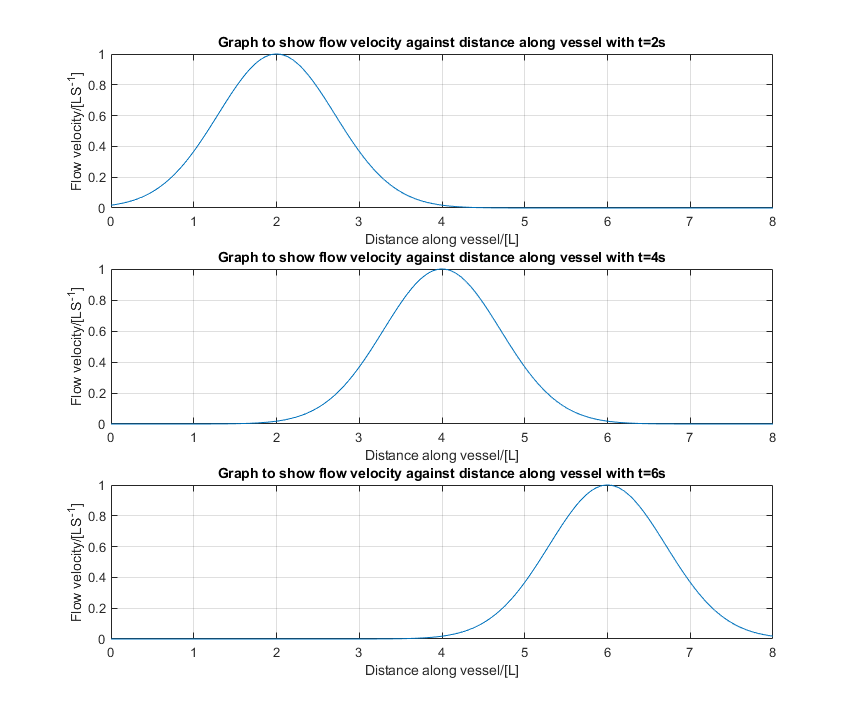
\includegraphics[width = \textwidth]{./img/q102b.png}
    \caption{Graphs to show and compare the effect of varying $t$ for flow velocity along the vessel.}
    \label{fig:q102a}
\end{figure}
\subsection{Constant cross-sectional area}
\subsubsection{Effect on $c$}
We know that:
\begin{equation}
    c = \frac{1}{S}\frac{\dif S}{\dif P}
\end{equation}
In the case where the cross-sectional area $S$ is constant, its derivative will be 0:
\begin{align}
    c &= \frac{1}{S} \cdot 0\\
    c &= 0
\end{align}
\subsubsection{Substitution}
We know that $c = 0$, hence:
\begin{align}
    \frac{\partial v}{\partial x} + gp &= 0 \label{eq:1.3.2a}\\
    \rho \frac{\partial v}{\partial t} + \frac{\partial p}{\partial x}+ rv &= 0 \label{eq:1.3.2b}
\end{align}
We also know the flow velocity $v$ is defined as:
\begin{equation}
    v = V e^{-\frac{rt}{\rho}}
\end{equation}
Differentiating $v$ with respect to $t$:
\begin{align}
    \frac{\partial }{\partial t} \left(V e^{-\frac{rt}{\rho}}\right) = \frac{\partial V }{\partial t} e^{-\frac{rt}{\rho}} - \frac{rV}{\rho} e^{-\frac{rt}{\rho}} \label{eq:1.3.2c}
\end{align}
Differentiating $v$ with respect to $x$:
\begin{equation}
    \frac{\partial }{\partial x} \left(V e^{-\frac{rt}{\rho}}\right) = \frac{\partial V}{\partial x} e^{-\frac{rt}{\rho}} \label{eq:1.3.2d}
\end{equation}
Substituting \ref{eq:1.3.2d} into \ref{eq:1.3.2a}:
\begin{gather}
    \frac{\partial V}{\partial x} e^{-\frac{rt}{\rho}} + gp = 0\\
    p = -\frac{1}{g}e^{-\frac{rt}{\rho}}\frac{\partial V}{\partial x}
\end{gather}
Differentiating with respect to $x$:
\begin{equation}
    \frac{\partial p}{\partial x} = - \frac{1}{g}e^{-\frac{rt}{\rho}}\frac{\partial^2 V}{\partial x^2} \label{eq:1.3.2e}
\end{equation}
Substituting \ref{eq:1.3.2c} and \ref{eq:1.3.2e} into \ref{eq:1.3.2b}:
\begin{gather}
    \rho\left(\frac{\partial V }{\partial t} e^{-\frac{rt}{\rho}} - \frac{rV}{\rho} e^{-\frac{rt}{\rho}}\right) - \frac{1}{g}e^{-\frac{rt}{\rho}}\frac{\partial^2 V}{\partial x^2} + r\left(V e^{-\frac{rt}{\rho}}\right) = 0
\end{gather}
Simplifying:
\begin{gather}
    \rho \frac{\partial V }{\partial t} e^{-\frac{rt}{\rho}} - rVe^{-\frac{rt}{\rho}}- \frac{1}{g}e^{-\frac{rt}{\rho}}\frac{\partial^2 V}{\partial x^2} + rVe^{-\frac{rt}{\rho}} = 0\\
    \rho \frac{\partial V }{\partial t} e^{-\frac{rt}{\rho}} = \frac{1}{g}e^{-\frac{rt}{\rho}}\frac{\partial^2 V}{\partial x^2}\\
    \frac{\partial V }{\partial t} = \frac{1}{g\rho}\frac{\partial^2 V}{\partial x^2}
\end{gather}
\subsection{Solving E6}
\subsubsection{Separation of variables}
Boundary conditions:
\begin{align}
    V(x,0) &= V_0 \cos\left(\frac{\pi x}{2l}\right) \textrm{ at } t=0 \textrm{ and for } 0 \leq x \leq l\\
    V(l,t) &= 0 \textrm{ at } x = l \textrm{ and for } t > 0\\
    V(0,t) &= V_0e^{-\frac{\pi^2 t}{4l^2}} \textrm{ at } x = 0 \textrm{ and for } t > 0
\end{align}
Starting with:
\begin{equation}
    \frac{\partial V}{\partial t} = \frac{1}{\rho g }\frac{\partial^2 V}{\partial x}
\end{equation}
We know that $\rho g = 1$:
\begin{equation}
    \frac{\partial V}{\partial t} = \frac{\partial^2 V}{\partial x}
\end{equation}
Assume that:
\begin{equation}
    V(x,t) = X(x)T(t)
\end{equation}
Substituting:
\begin{gather}
    X(x)T'(t) = X''(x)T(t)\\
    \frac{T'(t)}{T(t)} = \frac{X''(x)}{X(x)} = \lambda
\end{gather}
where $\lambda$ is a constant. Consider the case for $T$
\begin{gather}
    \frac{1}{T(t)}\frac{\dif T(t)}{\dif t} = \lambda\\
    \int \left(\frac{1}{T(t)}\frac{\dif T(t)}{\dif t}\right) \dif t = \int \left(\lambda \right) \dif t\\
    \ln\left(T(t)\right) = \lambda t + c\\
    T(t) = Ae^{\lambda t}
\end{gather}
We can consider three cases for the above. 

Case 1: $\lambda = 0$:
\begin{gather}
    X''(x) = 0\\
    X'(x) = a_1\\
    X(x) = a_1 x + a_2
\end{gather}
Therefore:
\begin{gather}
    V(x,t) = X(x)T(t)\\
    V(x,t) = \left(a_1 x + a_2\right)\left(Ae^0\right)\\
    V(x,t) = A a_1 x + Aa_2 
\end{gather}
Consider the third boundary condition:
\begin{align}
    V(0,t) &= V_0 e^{-\frac{\pi^2 t}{4l^2}}\\
    Aa_2 &= V_0 e^{-\frac{\pi^2 t}{4l^2}}
\end{align}
This only occurs at $t = 0$, hence the solution is trivial and does not contribute to the solution.

Case 2: $\lambda = \mu^2 > 0$
\begin{gather}
    \frac{X''(x)}{X(x)} = \mu^2\\
    X''(x) - \mu^2 X(x) = 0
\end{gather}
Solving the second order differential:
\begin{gather}
    m^2 = \mu^2\\
    m_1 = \mu, \; m_2 = - \mu\\
    X(x) = b_1 e^{\mu x } + b_2 e^{-\mu x}\\
    T(t) = Ae^{\mu^2 t}\\
    X(x)T(t) = \left(b_1 e^{\mu x } + b_2 e^{-\mu x}\right)Ae^{\mu^2 t}
\end{gather}
Consider the third boundary condition:
\begin{gather}
    V(0,t) = V_0 e^{-\frac{\pi^2 t}{4l^2}}\\
    \left(b_1 + b_2\right)Ae^{\mu^2 t} = V_0 e^{-\frac{\pi^2 t}{4l^2}}\\
    \therefore \mu^2 t = -\frac{\pi^2 t }{4l^2}\\
    \mu = \sqrt{-\frac{\pi^2 }{4l^2}}
\end{gather}
$\mu$ is complex and gives a trivial solution, which does not contribute to the solution.

Case 3: $\lambda = \mu^2 < 0$:
\begin{gather}
    X''(x) + \mu^2 X(x) = 0
\end{gather}
Solving the second order differential equation:
\begin{gather}
    m^2 = - \mu^2 \\
    m_1 = \mu i, \; m_2 = -\mu i
    X(x) = c_1 e^{i\mu x} + c_2 e^{-i\mu x}
\end{gather}
Using Euler's Formula:
\begin{gather}
    X(x) = c_3 \cos\mu x + c_4 \sin \mu x
\end{gather}
where $c_3 = c_1 + c_2$ and $c_4 = i\left(c_1 + c_2\right)$. Consider the third boundary condition:
\begin{gather}
    V(0,t) = V_0 e^{-\frac{\pi^2 t}{4l^2}}\\
    \left(c_3 \cos 0 + c_4 \sin 0\right)\left(Ae^{\lambda t}\right) = V_0 e^{-\frac{\pi^2 t}{4l^2}}\\
    c_3 A e^{\lambda t} = V_0 e^{-\frac{\pi^2 t}{4l^2}}\\
    \therefore \lambda t = - \frac{\pi^2 t}{4l^2}\\
\end{gather}
We know that $\mu < 0$, hence:
\begin{gather}
    \mu = \frac{\pi}{2l}
\end{gather}
Therefore:
\begin{gather}
    V(x,t) = X(x)T(t)\\
    V(x,t) = \left(d_1 \cos \mu x + d_2 \sin \mu x\right) e^{\lambda t}
\end{gather}
where $d_1 = Ac_1$ and $d_2 = Ac_2$. Consider the first boundary condition:
\begin{gather}
    V(x,0) = V_0 \cos \left(\frac{\pi x}{2l}\right)\\
    \left(d_1 \cos \mu x + d_2 \sin \mu x\right) e^{\lambda \cdot 0} = V_0 \cos \left(\frac{\pi x}{2l}\right)\\
    d_1 \cos \mu x + d_2 \sin \mu x = V_0 \cos \left(\frac{\pi x}{2l}\right)
\end{gather}
If $d_1 = V_0$ then $d_2 \sin \mu x = 0$, but we know that $\sin \mu x \neq 0$, leading to $d_2 = 0$. Consider the second boundary condition:
\begin{gather}
    V(l,t) = 0\\
    V(l,t) = V_0 \cos \left(\frac{\pi}{2}\right)e^{-\frac{\pi^2 t}{4l^2}}\\
    V(l,t) = V_0 \cdot 0 
\end{gather}
Hence, $V_0 \neq 0$ for a non-trivial solution. Hence:
\begin{gather}
    V(x,t) = V_0 \cos \left(\frac{\pi x}{2l}\right)e^{-\frac{\pi^2 t}{4l^2}}
\end{gather}
\subsubsection{Plot of $v$}
We know that:
\begin{gather}
    v = V e^{-\frac{rt}{\rho}}
\end{gather}
$\frac{r}{\rho} = 1$:
\begin{gather}
    v = Ve^{-t}\\
    v = V_0 \cos \left(\frac{\pi x}{2l}\right)e^{-\frac{\pi^2 t}{4l^2}} \cdot e^{-t}\\
    v =  V_0 \cos \left(\frac{\pi x}{2l}\right)e^{-t\left(1 + \frac{\pi^2}{4l^2}\right)}
\end{gather}
\lstset{language=Matlab,%
    %basicstyle=\color{red},
    breaklines=true,%
    morekeywords={matlab2tikz},
    keywordstyle=\color{blue},%
    morekeywords=[2]{1}, keywordstyle=[2]{\color{black}},
    identifierstyle=\color{black},%
    stringstyle=\color{mylilas},
    commentstyle=\color{mygreen},%
    showstringspaces=false,%without this there will be a symbol in the places where there is a space
    numbers=left,%
    numberstyle={\tiny \color{black}},% size of the numbers
    numbersep=9pt, % this defines how far the numbers are from the text
    emph=[1]{for,end,break},emphstyle=[1]\color{red}, %some words to emphasise
    %emph=[2]{word1,word2}, emphstyle=[2]{style},    
}
\lstinputlisting{./mCode/q104b.m}
\begin{figure}[H]
    \centering
    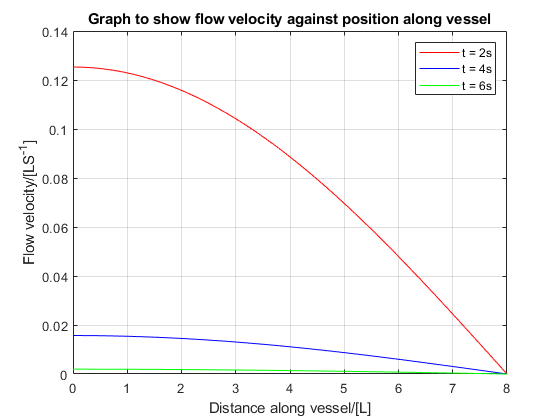
\includegraphics[height = 7cm]{./img/q104b.png}
    \caption{Graph of flow velocity against position in vessel for three values of $t$.}
    \label{fig:q104b}
\end{figure}
\subsection{Finite difference numerical scheme}
Starting with:
\begin{gather}
    \frac{\partial v}{\partial t} = \frac{1}{\rho g}\frac{\partial^2 v}{\partial x^2}
\end{gather}
$\rho g = 1$:
\begin{gather}
    \frac{\partial v}{\partial t} = \frac{\partial^2 v}{\partial x^2}
\end{gather}
We know that:
\begin{align}
    \frac{\partial v}{\partial t} &= \frac{u_{i,j}-u_{i,j-1}}{k}\\
    \frac{\partial^2 v}{\partial x^2} &= \frac{u_{i+1,j} -2u_{i,j} + u_{i-1,j}}{h^2}\\
    \therefore h^2 \left(u_{i,j} - u_{i,j-1}\right) &= k \left( u_{i+1,j} - 2u_{i,j} + u_{i-1,j} \right)
\end{align}
Expanding and simplifying:
\begin{gather}
    h^2 u_{i,j} + 2k u_{i,j} = h^2 u_{i,j-1} + k u_{i+1,j} + k u_{i-1,j}\\
    u_{i,j} = \frac{1}{h^2 +2k} \left(h^2 u_{i,j-1} + k u_{i+1,j} + k u_{i-1,j}\right)
\end{gather}
Using $h = k = 2$:
\begin{equation}
    u_{i,j} = \frac{1}{8} \left(4 u_{i,j-1} + 2 u_{i+1,j} + 2 u_{i-1,j}\right)
\end{equation}
\begin{figure}[H]
    \centering
    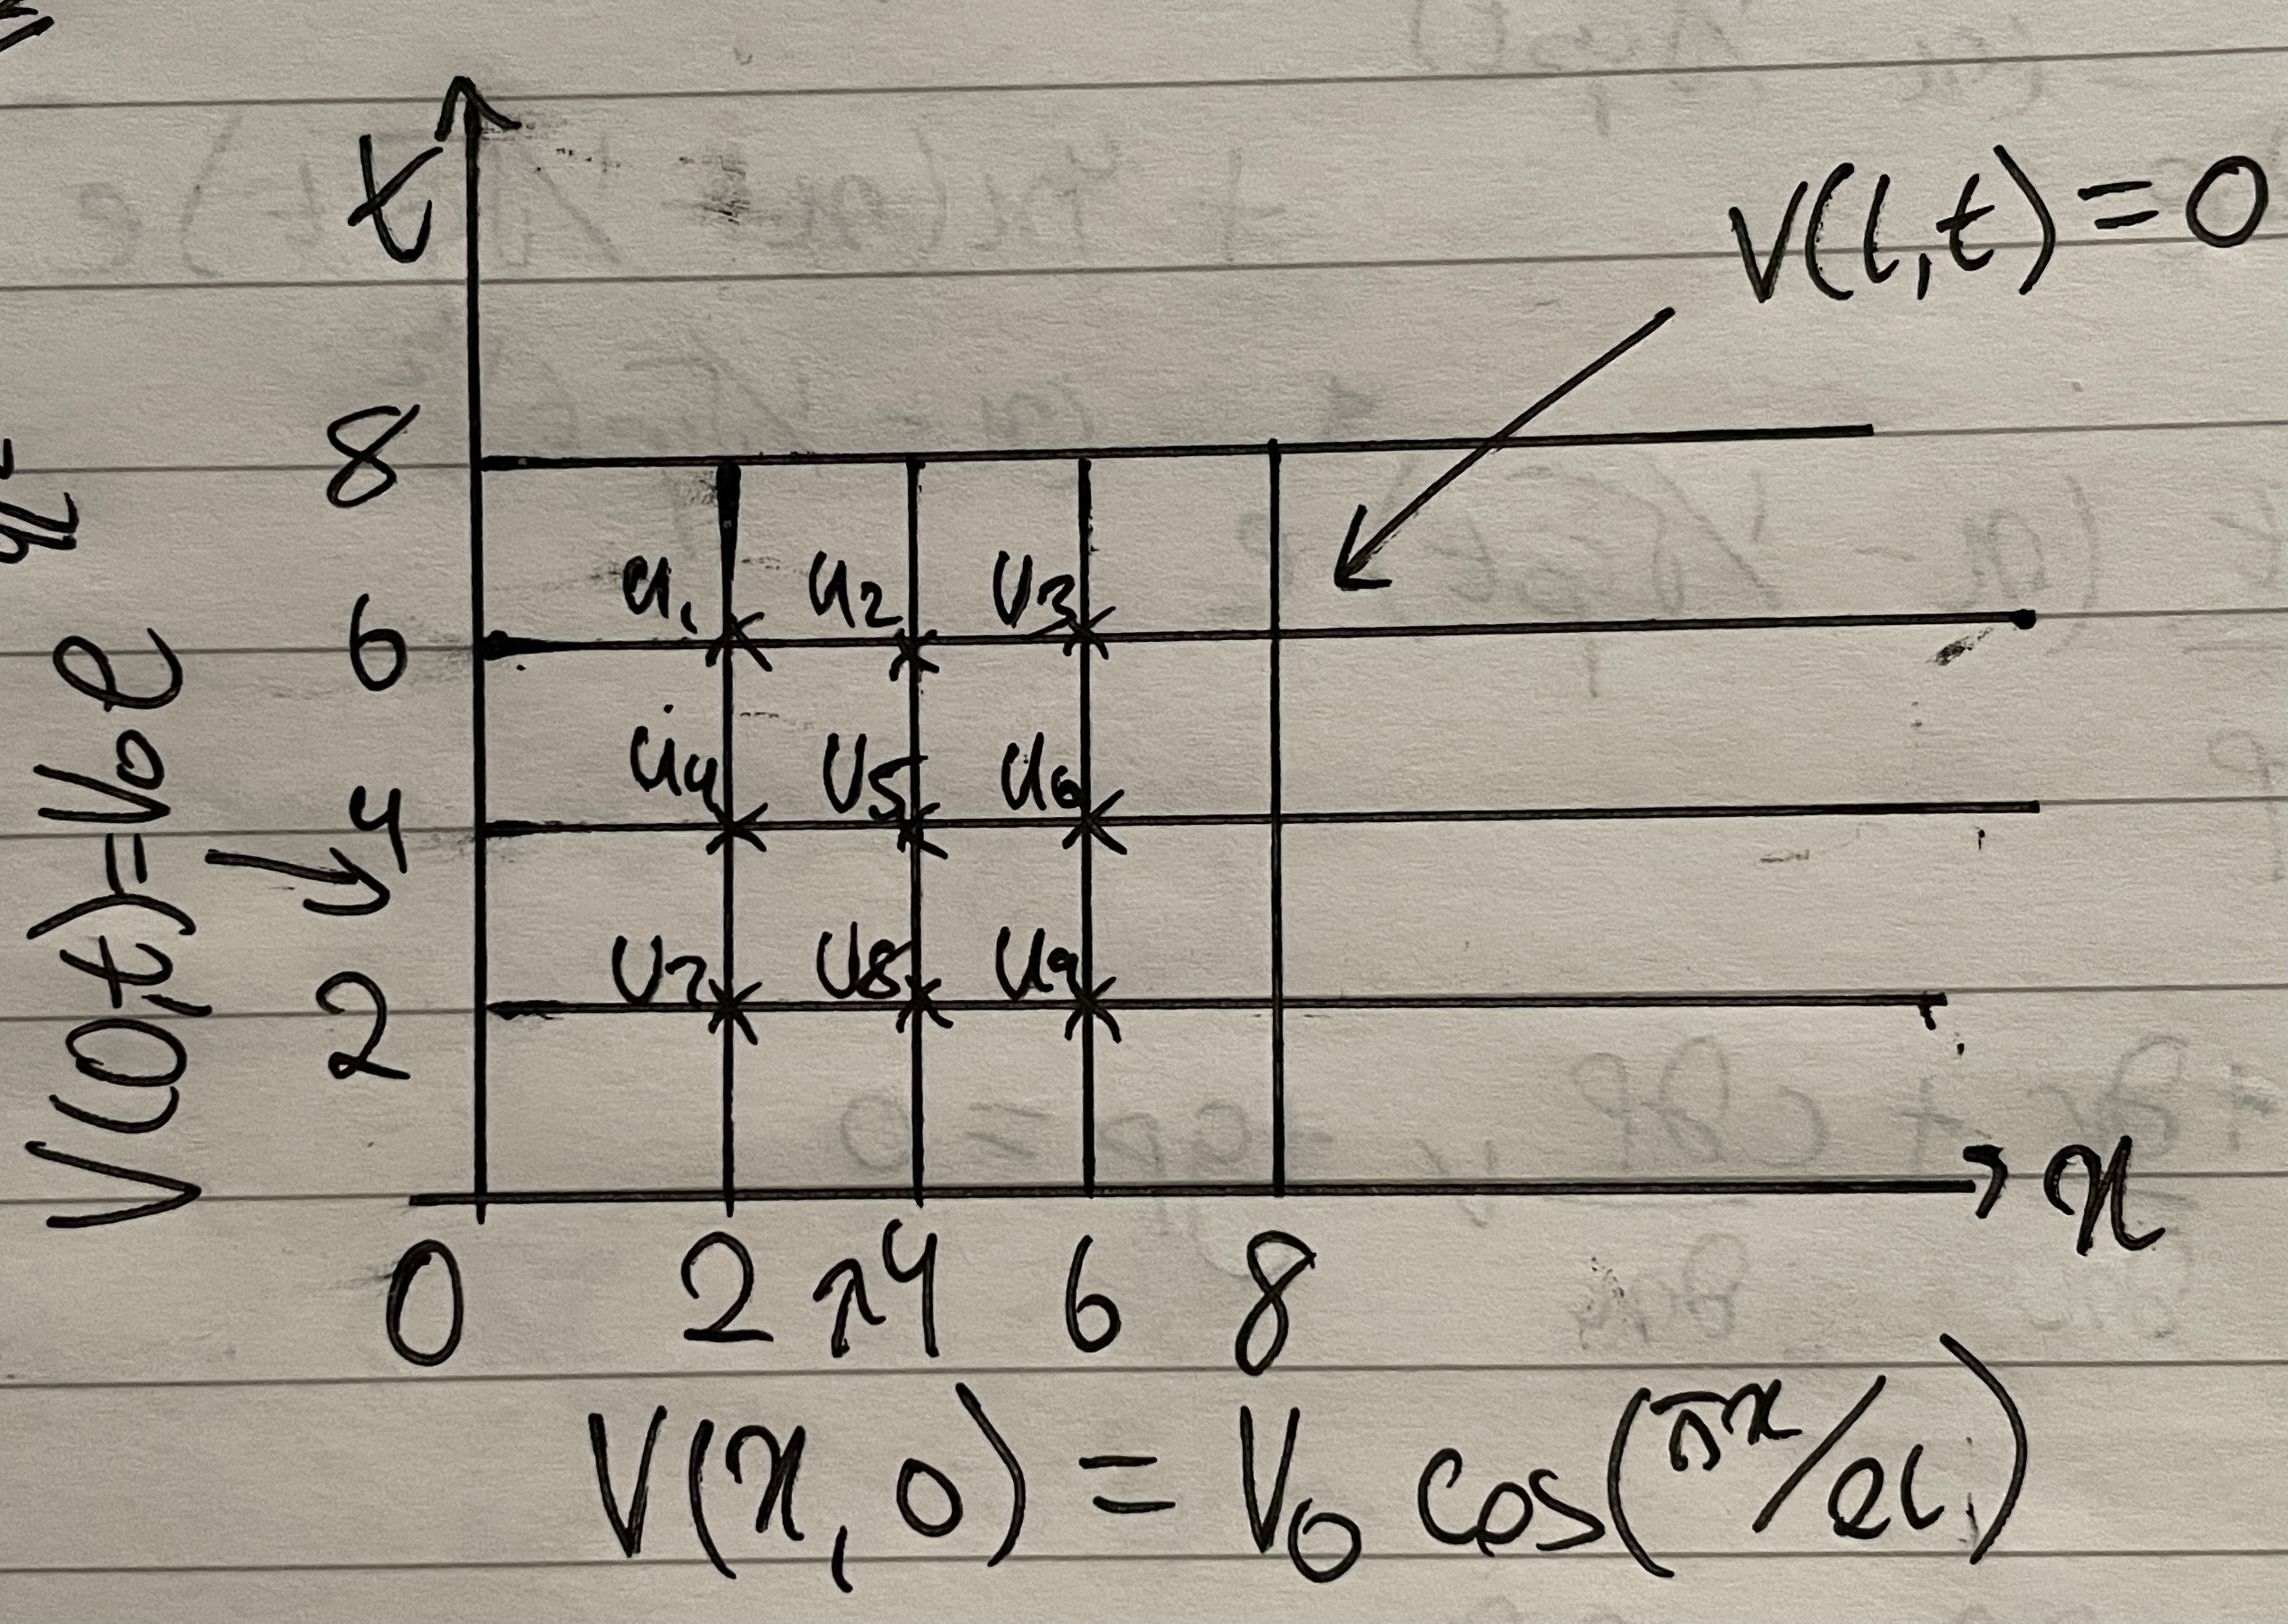
\includegraphics[height = 7cm]{./img/q105a.jpg}
    \caption{Sketch of domain.}
    \label{fig:q105a}
\end{figure}
Hence, our equations are:
\begin{align}
    u_1 &= \frac{1}{8}\left(4u_4 + 2u_2 + 2V_0 e^{-\frac{\pi^2 t }{4l^2}}\right)\\
    u_2 &= \frac{1}{8}\left(4u_5 + 2u_3 + 2u_1\right)\\
    u_3 &= \frac{1}{8}\left(4u_6 + 2(0) + 2u_2\right)\\
    u_4 &= \frac{1}{8}\left(4u_7 + 2u_5 + 2V_0 e^{-\frac{\pi^2 t }{4l^2}}\right)\\
    u_5 &= \frac{1}{8}\left(4u_8 + 2u_6 + 2u_4\right)\\
    u_6 &= \frac{1}{8}\left(4u_9 + 2(0) + 2u_5\right)\\
    u_7 &= \frac{1}{8}\left(4V_0\cos\left(\frac{\pi x}{2l}\right) + 2u_8 + 2V_0 e^{-\frac{\pi^2 t }{4l^2}}\right)\\
    u_8 &= \frac{1}{8}\left(4V_0\cos\left(\frac{\pi x}{2l}\right) + 2u_9 + 2u_7\right)\\
    u_9 &= \frac{1}{8}\left(4V_0\cos\left(\frac{\pi x}{2l}\right) + 2(0) + 2u_8\right)
\end{align}
Matrix:
\begin{gather}
    \begin{pmatrix}
        8 & -2 & 0 & -4 & 0 & 0 & 0 & 0 & 0\\ 
        -2 & 8 & -2 & 0 & -4 & 0 & 0 & 0 & 0\\ 
        0 & -2 & 8 & 0 & 0 & -4 & 0 & 0 & 0\\ 
        0 & 0 & 0 & 8 & -2 & 0 & -4 & 0 & 0\\ 
        0 & 0 & 0 & -2 & 8 & -2 & 0 & -4 & 0\\ 
        0 & 0 & 0 & 0 & -2 & 8 & 0 & 0 & -4\\ 
        0 & 0 & 0 & 0 & 0 & 0 & 8 & -2 & 0\\ 
        0 & 0 & 0 & 0 & 0 & 0 & -2 & 8 & -2\\
        0 & 0 & 0 & 0 & 0 & 0 & 0 & -2 & 8\\ 
    \end{pmatrix}  \begin{pmatrix}
        u_1 \\
        u_2 \\
        u_3 \\
        u_4 \\
        u_5 \\
        u_6 \\
        u_7 \\
        u_8 \\
        u_9
    \end{pmatrix} = \begin{pmatrix}
        2V_0e^{-\frac{\pi^2 t }{4l^2}}\\
        0\\
        0\\
        2V_0e^{-\frac{\pi^2 t }{4l^2}}\\
        0\\
        0\\
        4V_0 \cos \left(\frac{\pi x}{2l}\right) + 2V_0e^{-\frac{\pi^2 t }{4l^2}}\\
        4V_0 \cos \left(\frac{\pi x}{2l}\right) \\
        4V_0 \cos \left(\frac{\pi x}{2l}\right) 
    \end{pmatrix}
\end{gather}
\subsubsection{Implementation of numerical scheme in MATLAB}
\lstset{language=Matlab,%
    %basicstyle=\color{red},
    breaklines=true,%
    morekeywords={matlab2tikz},
    keywordstyle=\color{blue},%
    morekeywords=[2]{1}, keywordstyle=[2]{\color{black}},
    identifierstyle=\color{black},%
    stringstyle=\color{mylilas},
    commentstyle=\color{mygreen},%
    showstringspaces=false,%without this there will be a symbol in the places where there is a space
    numbers=left,%
    numberstyle={\tiny \color{black}},% size of the numbers
    numbersep=9pt, % this defines how far the numbers are from the text
    emph=[1]{for,end,break},emphstyle=[1]\color{red}, %some words to emphasise
    %emph=[2]{word1,word2}, emphstyle=[2]{style},    
}
\lstinputlisting{./mCode/q105b.m}
This gave the following output:
\begin{table}[H]
    \centering
    \begin{tabular}{llll}
        \toprule
        \textbf{Variable} & \textbf{Estimated value} & \textbf{Exact value} & \textbf{Percentage error}\\
        \midrule
        $u_1$ & 0.7376 & 0.7331 & 0.6212 \\
        $u_2$ & 0.5660 & 0.5611 & 0.8766 \\
        $u_3$ & 0.3066 & 0.3037 & 0.9769 \\
        $u_4$ & 0.7955 & 0.7918 & 0.4660 \\
        $u_5$ & 0.6099 & 0.6061 & 0.6289 \\
        $u_6$ & 0.3302 & 0.3280 & 0.6855 \\
        $u_7$ & 0.8576 & 0.8553 & 0.2663 \\
        $u_8$ & 0.6568 & 0.6546 & 0.3372 \\
        $u_9$ & 0.3556 & 0.3543 & 0.3576 \\ 
        \bottomrule
    \end{tabular}
    \caption{Table to show values of variables.}
\end{table}
From our percentage errors, we can see that no value exceeds an error of 1\%, hence we can say that the approximation is effective.
\subsection{Implications on stiffening blood vessel walls in the ageing population}
As a population ages, the stiffness of the blood vessel walls increases. For stretchy blood vessels, we see an effective transfer of blood (and oxygen) through the vessel. The flow velocity profile along the vessel is ideal as it transfers the velocity from one to the other end, as can be seen in Figure \ref{fig:q102a}. For a stiff blood vessel, the ability for the vessel to transfer the velocity of the fluid along its length is greatly reduced. Whereas previously, we had a wave travelling through the vessel, in a stiff blood vessel the blood is 'pushed' through the vessel ineffectively as the flow velocity is strictly decreasing. With time, the flow velocity decreases greatly and blood flow is reduced. In practical terms this lessened blood flow leads to hypertension \cite{q1.6.1}, causing high blood pressure as the heart cannot deliver oxygen to components around the body. This increases the risk of cardiovascular diseases such as strokes and aneurysms \cite{q1.6.2}.
\section{Vector calculus}
\subsection{Proof that divergence of velocity equals zero}
\begin{proof}
If the fluid is incompressible, our total derivative is zero:
\begin{align}
    \frac{\textrm{D}\rho}{\textrm{D}t} &= 0
\end{align}
We can start to derive the divergence of the velocity by rewriting the second term in \ref{eq2.1a}:
\begin{align}
    \frac{\partial \rho}{\partial t} + \nabla \cdot \left(\rho \underline{u}\right) &= 0 \label{eq2.1a}\\ 
    \frac{\partial \rho}{\partial t} + \rho \left(\nabla \cdot \underline{u}\right) + \underline{u} \cdot \left(\nabla \rho\right) &= 0
\end{align}
Looking at the $\nabla \rho$ term:
\begin{align}
    \nabla \rho = \left(\frac{\partial \rho}{\partial x}, \, \frac{\partial \rho}{\partial y}, \, \frac{\partial \rho}{\partial z}\right)
\end{align}
We know that all derivatives of $\rho$ are zero as $\rho$ is a constant, hence:
\begin{align}
    0 + \rho \left(\nabla \cdot \underline{u}\right) + 0 &= 0\\
    \nabla \cdot \underline{u} &= 0
\end{align}
\end{proof}
\subsection{Acceleration of fluid element}
Fluid element acceleration is given by:
\begin{equation}
    \frac{\textrm{D}u}{\textrm{D}t} = \frac{\partial \underline{u}}{\partial t} + \left(\underline{u}\cdot \nabla\right)\underline{u}
\end{equation}
Flow is steady, hence
\begin{align}
    \frac{\textrm{D}u}{\textrm{D}t} &= 0 + \left(\underline{u}\cdot \nabla\right)\underline{u}\\
    &= -\omega y\frac{\partial \underline{u}}{\partial x} + -\omega x \frac{\partial \underline{u}}{\partial y} + 0 \frac{\partial \underline{u}}{\partial z}\\
    &= -\omega y\frac{\partial \underline{u}}{\partial x} + \omega x \frac{\partial \underline{u}}{\partial x} \\
    &= -\omega y \begin{pmatrix}
        0\\
        \omega\\
        0
    \end{pmatrix} + \omega x \begin{pmatrix}
        -\omega\\
        0\\
        0
    \end{pmatrix}\\
    &= \begin{pmatrix}
        -\omega^2 x\\
        -\omega^2 y\\
        0
    \end{pmatrix}
\end{align}
\subsection{Integral}
Considering the volume of an element $V$, where $V$ is the region bounded by the planes $x=0$, $y=0$, $z=0$ and $x+y+z=1$:
\begin{equation}
    \iiint\displaylimits_V \left(xyz\right)\dif z \dif y \dif x\\
\end{equation}
\subsubsection{Area of integration}
\begin{figure}[H]
    \centering
    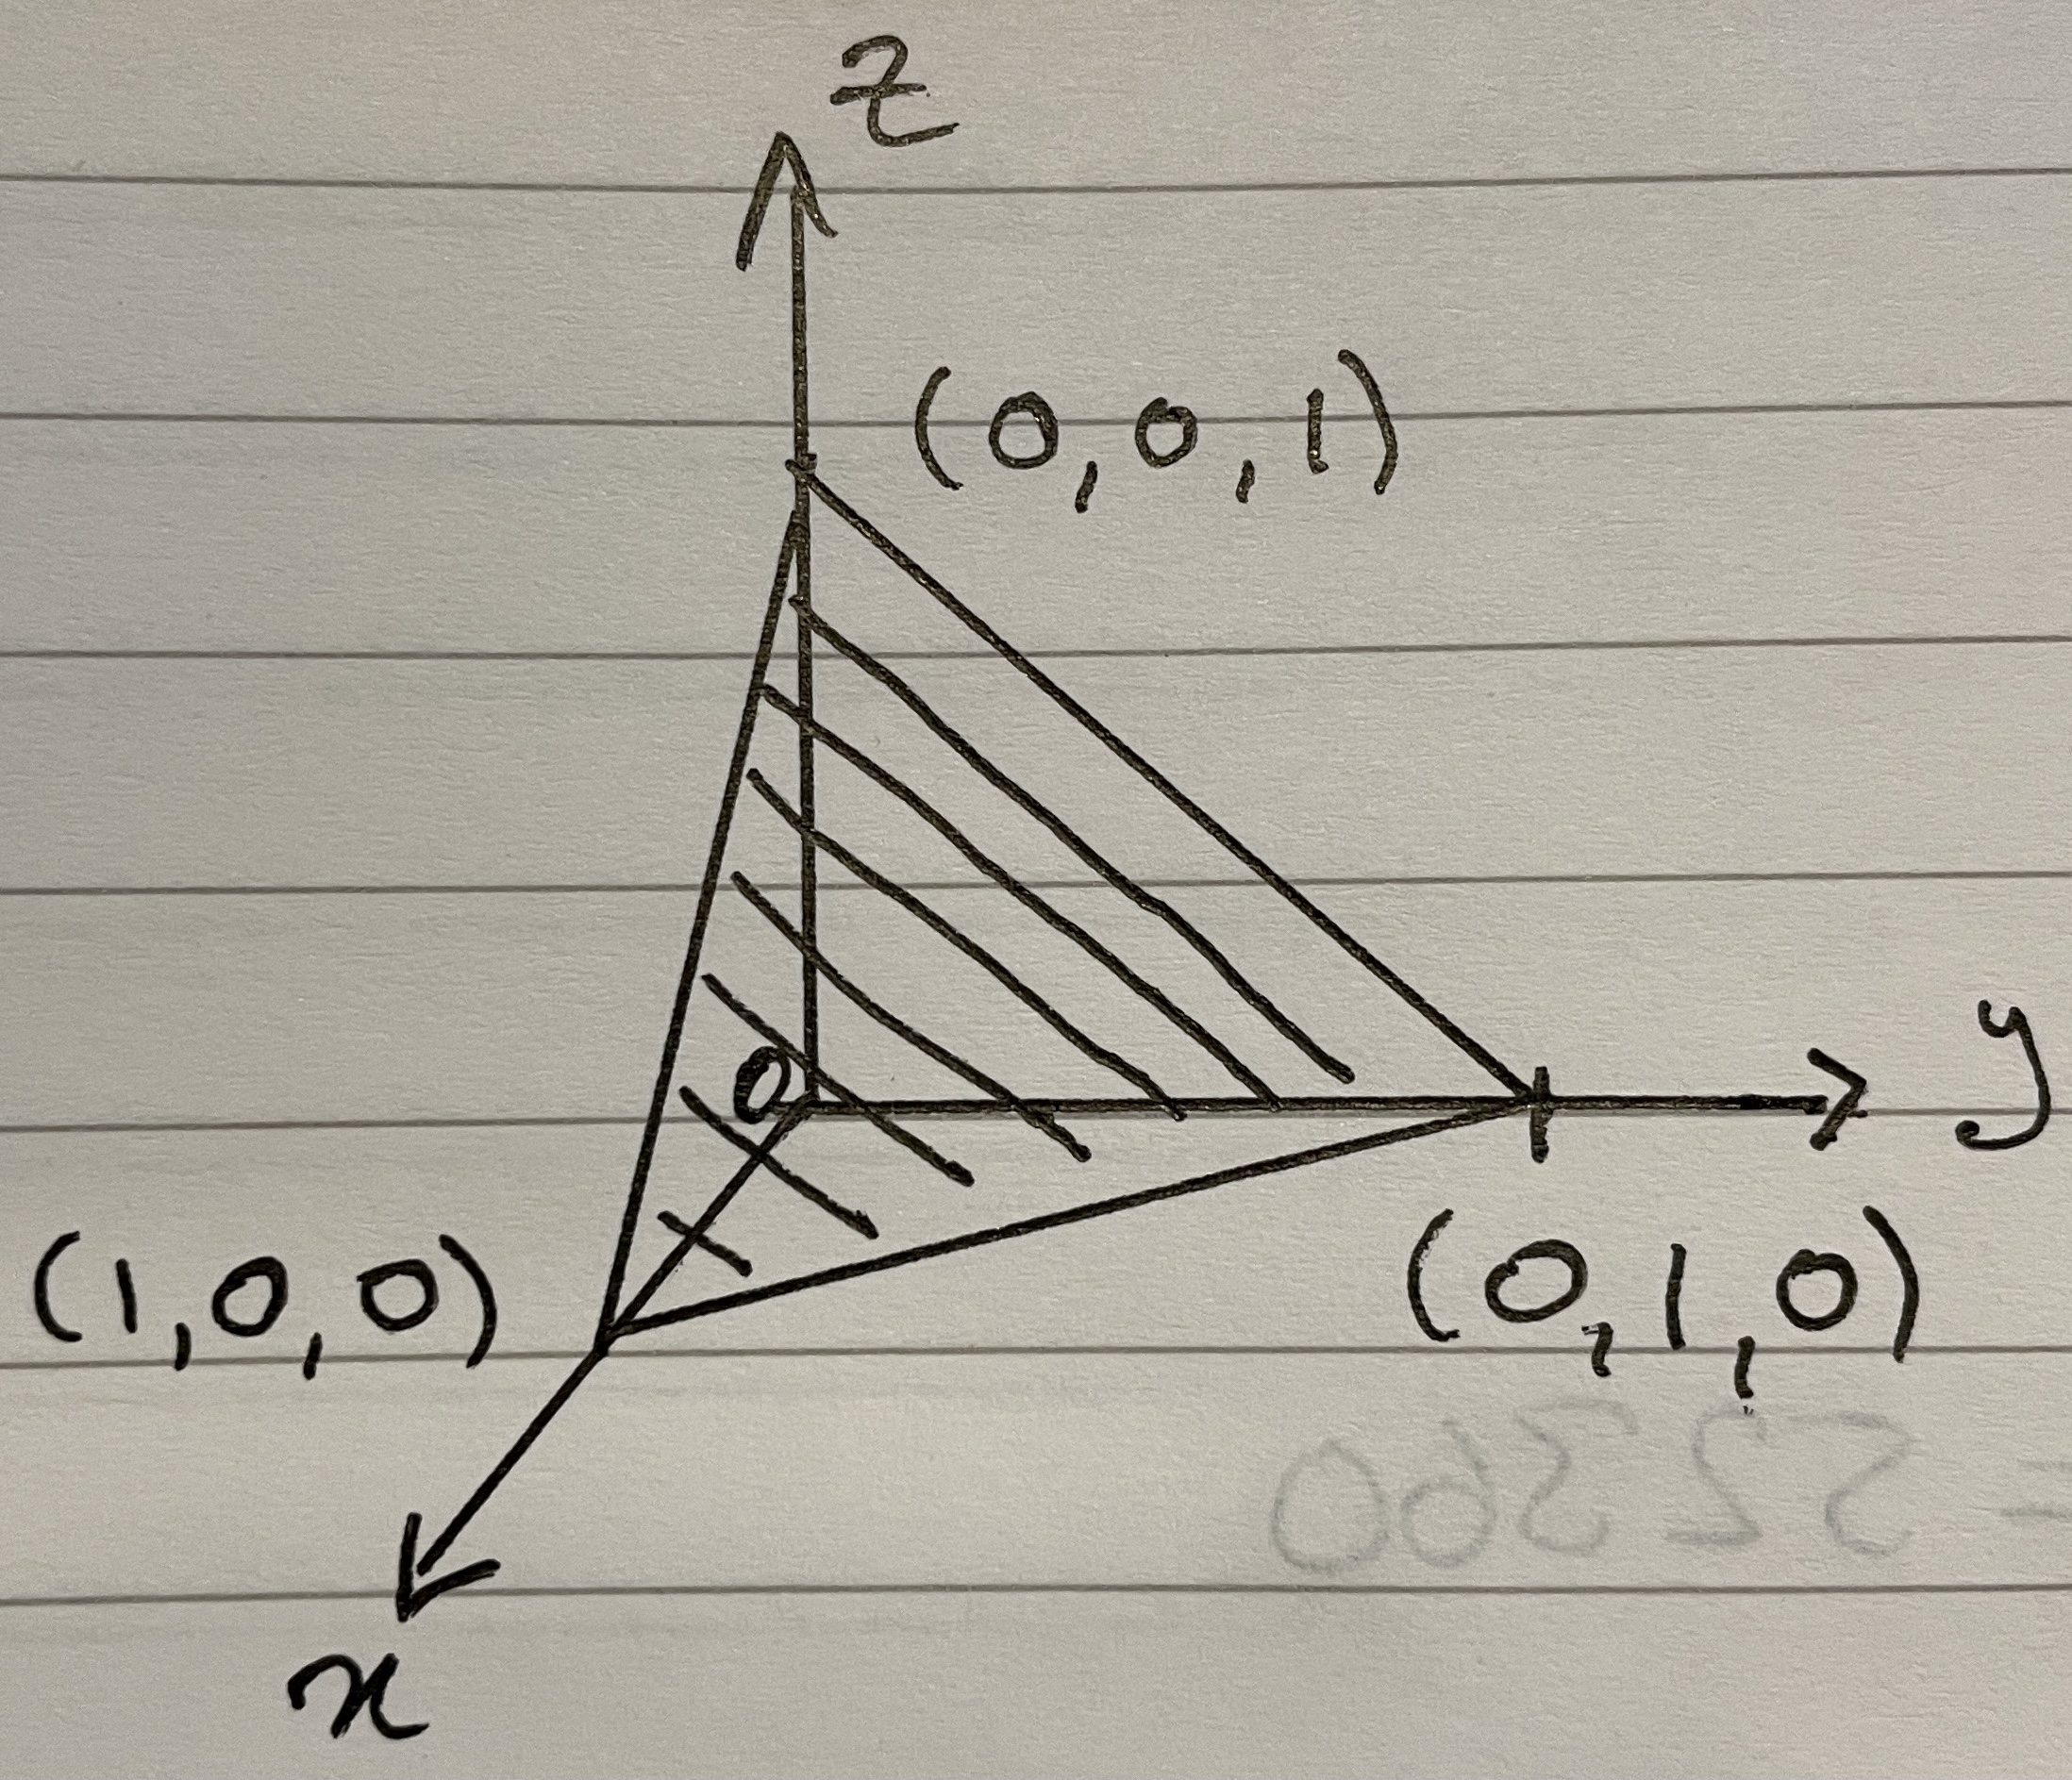
\includegraphics[height = 7cm]{./img/q203a.jpg}
    \caption{Graph to show area of integration of function.}
\end{figure}
\subsubsection{Find the limits of integration}
We know the volume is bounded by the $x$-$y$, $x$-$z$ and $y$-$z$ planes. Hence, our lower limits are:
\begin{align}
    x = 0, \; y = 0, \; z = 0
\end{align}
Our upper bound is $x+y+z \leq 1$. Hence, the upper bound for $z$ is:
\begin{gather}
    x + y + z \leq 1\\
    z \leq 1 - x - y
\end{gather}
Upper bound for $y$ ($x$-$y$ plane $\rightarrow z = 0$):
\begin{gather}
    x + y \leq 1\\
    y \leq 1 - x
\end{gather}
Upper bound for $x$ ($y=z=0$)
\begin{gather}
    x \leq 1
\end{gather}
\subsubsection{Calculation of triple integral}
\begin{equation}
    \int_0^1 \int_0^{1-x} \int_0^{1-x-y} \left(xyz\right)\dif z \dif y \dif x \label{q2.3a}
\end{equation}
Computing the $z$ integral:
\begin{align}
    &= xy\int_0^{1-x-y} \left(z\right)\dif z\\
    &= xy \left[\frac{z^2}{2}\right]_0^{1-x-y}\\
    &= xy \left[\frac{(1-x-y)^2}{2}-\frac{0^2}{2}\right]\\
    &= \frac{xy}{2} \left(y^2 + x^2 + 2xy -2x -2y + 1\right)\\
    &= \frac{1}{2}\left(xy^3 + x^3y + 2x^2 y^2 -2x^2y - 2y^2x + xy\right) \label{q2.3b}
\end{align}
Inputting \ref{q2.3b} into \ref{q2.3a}:
\begin{align}
    \int_0^1 \int_0^{1-x} \left(\frac{1}{2}\left(xy^3 + x^3y + 2x^2 y^2 -2x^2y - 2xy^2 + xy\right) \right)\dif y \dif x \label{q2.3d}
\end{align}
Computing the $y$ integral:
\begin{align}
    &= \frac{1}{2} \int_0^{1-x}\left(xy^3 + x^3y + 2x^2 y^2 -2x^2y - 2xy^2 + xy\right) \dif y\\
    &= \frac{1}{2}\left[\frac{xy^4}{4} + \frac{x^3y^2}{2} + \frac{2x^2y^3}{3} -x^2y^2-\frac{2xy^3}{3}+ \frac{xy^2}{2}\right]_0^{1-x}\\
    &= \frac{1}{2}\left[\frac{x\left(1-x\right)^4}{4} + \frac{x^3\left(1-x\right)^2}{2} + \frac{2x^2\left(1-x\right)^3}{3} -x^2\left(1-x\right)^2-\frac{2x\left(1-x\right)^3}{3}+ \frac{x\left(1-x\right)^2}{2}\right]
\end{align}
Expanding:
\begin{multline}
    = \frac{1}{2}\left[\frac{x - 4x^2 + 6x^3 - 4x^4 + x^5}{4} \right.+ \frac{x^3 - 2x^4 + x^5}{2} + \frac{2x^2-6x^3 + 6x^4 -2x^5}{3}\\ \left. -\left(x^2-2x^3+x^4\right)-\frac{2x-6x^2 +6x^3 -2x^4}{3}+ \frac{x-2x^2 + x^3}{2}\right]
\end{multline}
Simplifying
\begin{align}
    &= \frac{x^5 -4x^4 + 6x^3 -4x^2 + x}{24}\\
    &= \frac{1}{24}\left(x^5 -4x^4 +6x^3 -4x^2 + x\right) \label{q2.3c}
\end{align}
Inputting \ref{q2.3c} into \ref{q2.3d}:
\begin{equation}
    \int_0^1 \left( \frac{1}{24}\left(x^5 -4x^4 +6x^3 -4x^2 + x\right) \right)\dif x 
\end{equation}
Computing the $x$ integral:
\begin{align}
    &= \frac{1}{24}\left[\frac{x^6}{6}-\frac{4x^5}{5}+\frac{3x^4}{2}-\frac{4x^3}{3} + \frac{x^2}{2}\right]_0^1\\
    &= \frac{1}{24}\left[\frac{1}{6} - \frac{4}{5} + \frac{3}{2} - \frac{4}{3} + \frac{1}{2}\right]\\
    &= \frac{1}{720}
\end{align}
\section{Transforms}
\subsection{Plot of data}
\lstset{language=Matlab,%
    %basicstyle=\color{red},
    breaklines=true,%
    morekeywords={matlab2tikz},
    keywordstyle=\color{blue},%
    morekeywords=[2]{1}, keywordstyle=[2]{\color{black}},
    identifierstyle=\color{black},%
    stringstyle=\color{mylilas},
    commentstyle=\color{mygreen},%
    showstringspaces=false,%without this there will be a symbol in the places where there is a space
    numbers=left,%
    numberstyle={\tiny \color{black}},% size of the numbers
    numbersep=9pt, % this defines how far the numbers are from the text
    emph=[1]{for,end,break},emphstyle=[1]\color{red}, %some words to emphasise
    %emph=[2]{word1,word2}, emphstyle=[2]{style},    
}
\lstinputlisting{./mCode/q301a.m}
\begin{figure}[H]
    \centering
    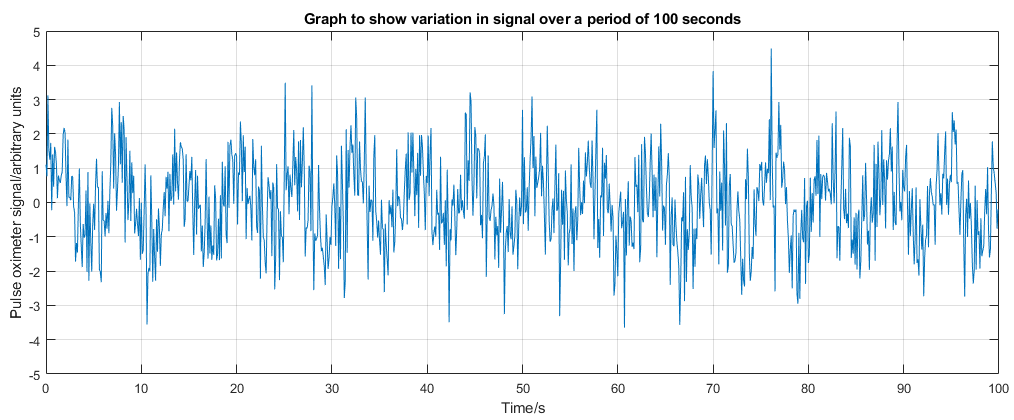
\includegraphics[width = \textwidth]{./img/q301a.png}
    \caption{Graph to show variation in signal over a period of 100 seconds.}
\end{figure}
\subsection{Plot of Fourier transform}
\lstset{language=Matlab,%
    %basicstyle=\color{red},
    breaklines=true,%
    morekeywords={matlab2tikz},
    keywordstyle=\color{blue},%
    morekeywords=[2]{1}, keywordstyle=[2]{\color{black}},
    identifierstyle=\color{black},%
    stringstyle=\color{mylilas},
    commentstyle=\color{mygreen},%
    showstringspaces=false,%without this there will be a symbol in the places where there is a space
    numbers=left,%
    numberstyle={\tiny \color{black}},% size of the numbers
    numbersep=9pt, % this defines how far the numbers are from the text
    emph=[1]{for,end,break},emphstyle=[1]\color{red}, %some words to emphasise
    %emph=[2]{word1,word2}, emphstyle=[2]{style},    
}
\lstinputlisting{./mCode/q302a.m}
\begin{figure}[H]
    \centering
    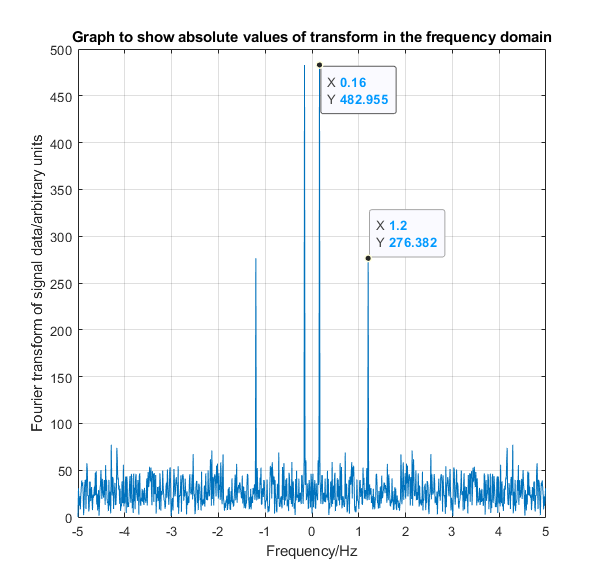
\includegraphics[height = 10cm]{./img/q302a.png}
    \caption{Graph to show absolute values of transform in the frequency domain.}
    \label{fig:q302a}
\end{figure}
\subsection{Extraction of patient's cardiac and respiratory cycle}
As seen from Figure \ref{fig:q302a}, we can extract two values from our Fourier transform. The higher peak has a frequency of \SI{0.16}{\hertz} and a period of \SI{6.25}{\second}. This represents the breathing of the subject (9.6 breaths per minute). According to a Cleveland Clinic article on vital signs, the average human breathing rate for adults should be around 12-16 breaths per minute \cite{q3.3.1}. The lower peak has a frequency of \SI{1.2}{\hertz} and a period of \SI{0.83}{\second}. This represents the heartbeat of the subject (72 beats per minute). According to the British Heart Foundation, the average resting heart rate for adults is between 60-100 beats per minute \cite{q3.3.2}.
\subsection{Frequency filter}
\subsubsection{Gaussian functions}
A Gaussian function is defined below as:
\begin{equation}
    f(x,\sigma,\mu) = \frac{1}{\sigma\sqrt{2\pi}}e^{-\frac{1}{2}\frac{\left(x - \mu\right)^2}{\sigma^2}}
\end{equation}
Here $\mu$ determines where the peak of our curve is and $\sigma$ determines the 'width' of our curve. We want to set $\mu$ to 1.2 and -1.2 to focus on the cardiac signal. We also want our standard deviation to be low, as to generate narrow peaks. We shall be utilising a special form of the Gaussian function for our filters which always has a maximum value of 1. This is called a Gaussian membership function and has the equation:
\begin{equation}
    f(x,\sigma,\mu) = e^{-\frac{1}{2}\frac{\left(x - \mu\right)^2}{\sigma^2}}
\end{equation}
A Gaussian membership function was generated using MATLAB's "gaussmf" function in the 'Fuzzy logic toolbox' \cite{q3.4.1}. $\mu = \pm1.2$. $\sigma = 0.01$ was selected arbitrarily to de-noise the signal to an appropriate level.
\lstset{language=Matlab,%
    %basicstyle=\color{red},
    breaklines=true,%
    morekeywords={matlab2tikz},
    keywordstyle=\color{blue},%
    morekeywords=[2]{1}, keywordstyle=[2]{\color{black}},
    identifierstyle=\color{black},%
    stringstyle=\color{mylilas},
    commentstyle=\color{mygreen},%
    showstringspaces=false,%without this there will be a symbol in the places where there is a space
    numbers=left,%
    numberstyle={\tiny \color{black}},% size of the numbers
    numbersep=9pt, % this defines how far the numbers are from the text
    emph=[1]{for,end,break},emphstyle=[1]\color{red}, %some words to emphasise
    %emph=[2]{word1,word2}, emphstyle=[2]{style},    
}
\lstinputlisting{./mCode/q304a.m}
\begin{figure}[H]
    \centering
    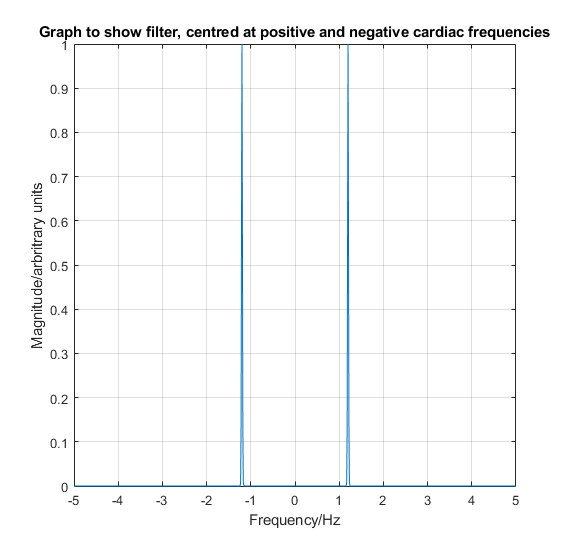
\includegraphics[height = 10cm]{./img/q304a.png}
    \caption{Graph to show filter, centred at positive and negative cardiac frequencies.}
    \label{fig:q304a}
\end{figure}
\subsubsection{Filtered/unfiltered Fourier data comparison}
\lstset{language=Matlab,%
    %basicstyle=\color{red},
    breaklines=true,%
    morekeywords={matlab2tikz},
    keywordstyle=\color{blue},%
    morekeywords=[2]{1}, keywordstyle=[2]{\color{black}},
    identifierstyle=\color{black},%
    stringstyle=\color{mylilas},
    commentstyle=\color{mygreen},%
    showstringspaces=false,%without this there will be a symbol in the places where there is a space
    numbers=left,%
    numberstyle={\tiny \color{black}},% size of the numbers
    numbersep=9pt, % this defines how far the numbers are from the text
    emph=[1]{for,end,break},emphstyle=[1]\color{red}, %some words to emphasise
    %emph=[2]{word1,word2}, emphstyle=[2]{style},    
}
\lstinputlisting{./mCode/q304b.m}
\begin{figure}[H]
    \centering
    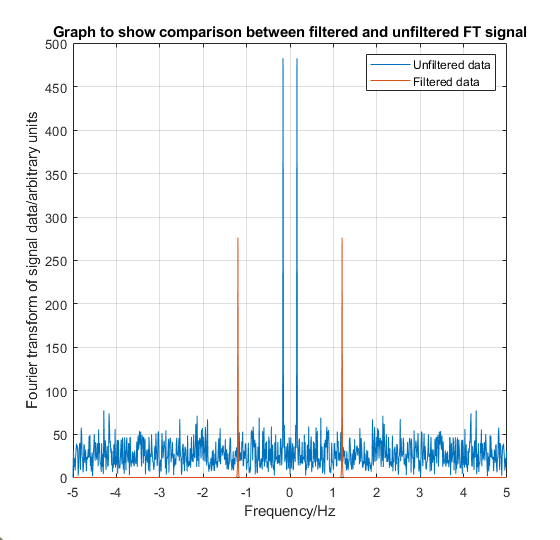
\includegraphics[height = 9cm]{./img/q304b.png}
    \caption{Graph to show comparison between filtered and unfiltered FT signal.}
    \label{fig:q304b}
\end{figure}
\begin{figure}[H]
    \centering
    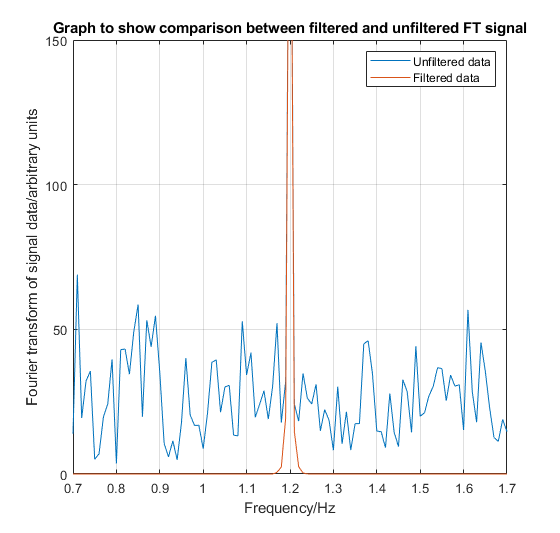
\includegraphics[height = 9cm]{./img/q304b2.png}
    \caption{Graph to show comparison between filtered and unfiltered FT signal (close-up).}
    \label{fig:q304b2}
\end{figure}
\subsection{Filtered data}
\lstset{language=Matlab,%
    %basicstyle=\color{red},
    breaklines=true,%
    morekeywords={matlab2tikz},
    keywordstyle=\color{blue},%
    morekeywords=[2]{1}, keywordstyle=[2]{\color{black}},
    identifierstyle=\color{black},%
    stringstyle=\color{mylilas},
    commentstyle=\color{mygreen},%
    showstringspaces=false,%without this there will be a symbol in the places where there is a space
    numbers=left,%
    numberstyle={\tiny \color{black}},% size of the numbers
    numbersep=9pt, % this defines how far the numbers are from the text
    emph=[1]{for,end,break},emphstyle=[1]\color{red}, %some words to emphasise
    %emph=[2]{word1,word2}, emphstyle=[2]{style},    
}
\lstinputlisting{./mCode/q305a.m}
\begin{figure}[H]
    \centering
    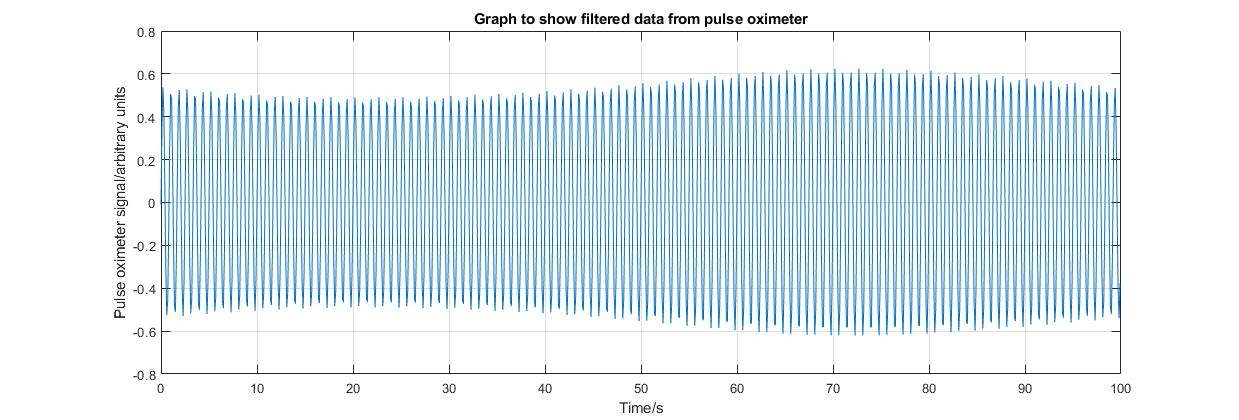
\includegraphics[width = \textwidth]{./img/q305a.png}
    \caption{Graph to show filtered data from pulse oximeter.}
    \label{fig:q305a}
\end{figure}
\subsection{Effect of varying the width of Gaussian function}
The code was adjusted to created two additional cases, to make four in total:
\begin{itemize}
    \item Unfiltered data
    \item Gaussian filter with $\sigma = 0.1$
    \item Gaussian filter with $\sigma = 0.01$
    \item Gaussian filter with $\sigma = 0.001$
\end{itemize}
\lstset{language=Matlab,%
    %basicstyle=\color{red},
    breaklines=true,%
    morekeywords={matlab2tikz},
    keywordstyle=\color{blue},%
    morekeywords=[2]{1}, keywordstyle=[2]{\color{black}},
    identifierstyle=\color{black},%
    stringstyle=\color{mylilas},
    commentstyle=\color{mygreen},%
    showstringspaces=false,%without this there will be a symbol in the places where there is a space
    numbers=left,%
    numberstyle={\tiny \color{black}},% size of the numbers
    numbersep=9pt, % this defines how far the numbers are from the text
    emph=[1]{for,end,break},emphstyle=[1]\color{red}, %some words to emphasise
    %emph=[2]{word1,word2}, emphstyle=[2]{style},    
}
\lstinputlisting{./mCode/q306a.m}
\begin{figure}[H]
    \centering
    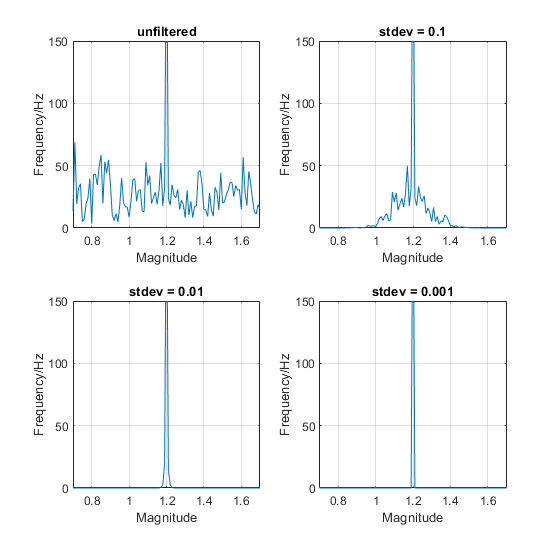
\includegraphics[width = \textwidth]{./img/q306a.png}
    \caption{Graphs to compare the effect of varying Gaussian filter width on FT signal.}
    \label{fig:q306a}
\end{figure}
Here we can see that adjusting the value of $\sigma$ effects the amount of noise that appears at the base of the peak in the Fourier transformed data. For $\sigma = 0.1$, there is still quite a bit of residual noise. $\sigma = 0.01$ and $\sigma = 0.001$ both do not exhibit any noise at the base, but we can see that for $\sigma = 0.01$, there is a slight flaring at the base.
\begin{figure}[H]
    \centering
    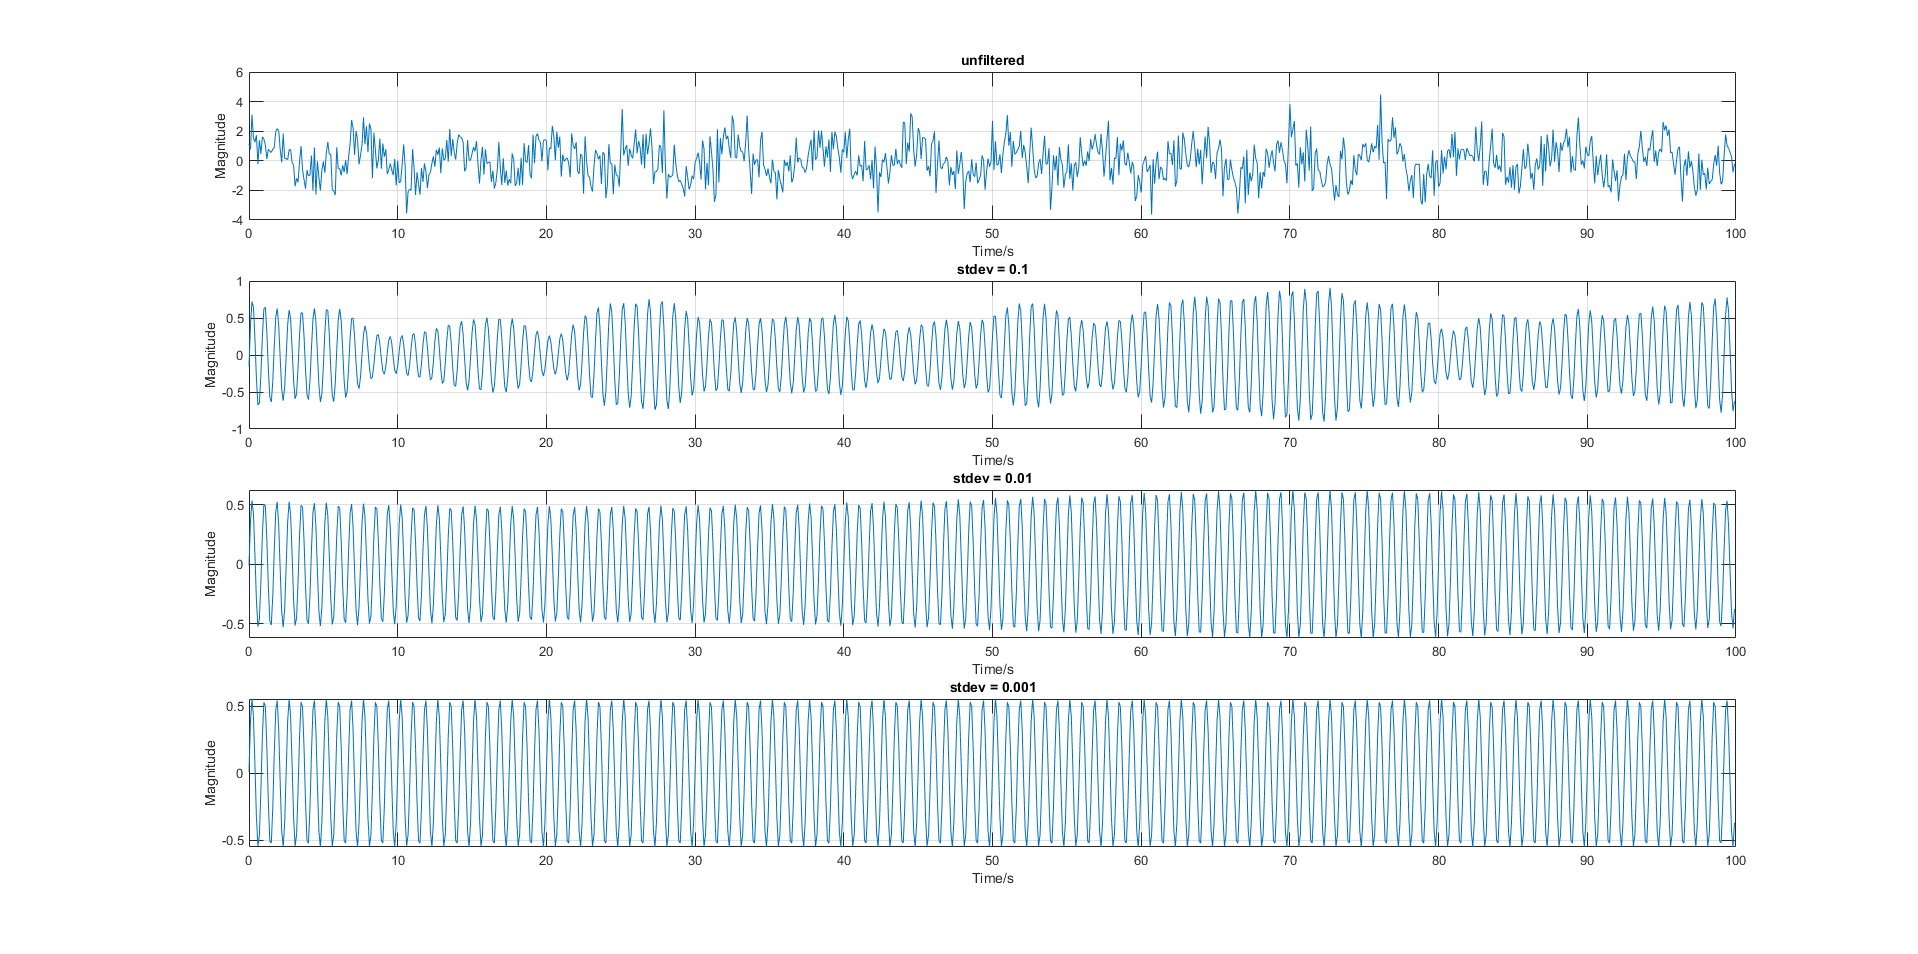
\includegraphics[width = \textwidth]{./img/q306b.png}
    \caption{Graphs to compare the effect of varying Gaussian filter width on signal from pulse oximeter.}
    \label{fig:q306b}
\end{figure}
Here we can see the effect of the residual noise in the $\sigma = 0.1$ case, with relatively large variations in the amplitude of the signal. We can also see the effect of the flared base in the $\sigma = 0.01$ case as a smooth decrease and then increase in the amplitude of the signal. The $\sigma = 0.001$ case represents a virtually perfect signal with a frequency of \SI{1.2}{\hertz}.
\section{Statistics}
\subsection{Confidence interval}
Formula for calculating mean:
\begin{equation}
    \bar{x} = \sum_{i = 1}^n\frac{x_i}{n}
\end{equation}
Formula for sample standard deviation:
\begin{equation}
    \sigma = \sqrt{\sum_{i = 1}^n \frac{\left(\bar{x} - x_i\right)^2}{n - 1}}
\end{equation}
\lstset{language=Matlab,%
    %basicstyle=\color{red},
    breaklines=true,%
    morekeywords={matlab2tikz},
    keywordstyle=\color{blue},%
    morekeywords=[2]{1}, keywordstyle=[2]{\color{black}},
    identifierstyle=\color{black},%
    stringstyle=\color{mylilas},
    commentstyle=\color{mygreen},%
    showstringspaces=false,%without this there will be a symbol in the places where there is a space
    numbers=left,%
    numberstyle={\tiny \color{black}},% size of the numbers
    numbersep=9pt, % this defines how far the numbers are from the text
    emph=[1]{for,end,break},emphstyle=[1]\color{red}, %some words to emphasise
    %emph=[2]{word1,word2}, emphstyle=[2]{style},    
}
\lstinputlisting{./mCode/q401a.m}
\begin{table}[H]
    \centering
    \begin{tabular}{lll}
        \toprule
        & \textbf{Rest} & \textbf{Anticipation}\\
        \midrule
        $n$ & 38 & 42\\
        Mean & 86.7368 & 92.4048 \\
        Standard deviation & 11.2842 & 16.6177\\
        \bottomrule
    \end{tabular}
    \caption{Table to show values of number of elements, means and standard deviations of heart rate data.}
\end{table}
A 95\% confidence interval can be found using \ref{eq:q401a}. A subscript of 1 represents the 'Rest' sample and a subscript of 2 represents the 'Anticipation' sample:
\begin{equation}
    CI = \bar{x}_1 - \bar{x}_2 \pm z_{crit} \sqrt{\frac{\sigma_1^2}{n_1} + \frac{\sigma_2^2}{n_2}} \label{eq:q401a}
\end{equation}
$z_{crit} = 1.96$ for a 95\% confidence interval in a two-tailed test, hence:
\begin{gather}
    CI = 86.7368 - 92.4048 \pm 1.96 \sqrt{\frac{11.2842^2}{38} + \frac{16.6177^2}{42}}\\
    CI_L = -11.84 \hspace{1cm} CI_H = 0.51
\end{gather} 
We can say with 95\% confidence that the true population mean's difference is in the interval [-11.85, 0.51]. This interval contains 0, hence we can deduce that there is not a significant indication of the means being different in this case. 

However, if we reduce our $z_{crit}$ value to 90\% ($z_{crit} = 1.65$):
\begin{gather}
    CI = 86.7368 - 92.4048 \pm 1.65 \sqrt{\frac{11.2842^2}{38} + \frac{16.6177^2}{42}}\\
    CI_L = -10.90 \hspace{1cm} CI_H = -0.43
\end{gather} 
This confidence interval does not contain 0, hence we could make the deduction that there is a significant difference at 90\% confidence interval.
\subsection{Reasoning for choice of test statistics}
\begin{itemize}
    \item We have assumed that a normal distribution applies in this case. Our sample sizes are larger than 30 in both cases, making the normal distribution a good approximation.
    \item A two-tailed test is used to account for both possibilities of difference. 
    \item The Central Limit Theorem allows us to approximate the sample's variance to the population's.
    \item We can use a z-test as our sample sizes are sufficiently large and independent. 
    \item A t-test does not apply as standard deviation is know and our sample size is not small.
\end{itemize}
\subsection{Hypothesis test}
Despite not knowing the true population standard deviation, we shall use a two-tailed two-sample z-test as our sample size is sufficiently large, as assuming the normal distribution will give us a good approximation. 
\begin{itemize}
    \item Null hypothesis: there is no difference between the true populations means of the rest and anticipation heart rates.
    \item Alternative hypothesis: there is a difference between the true population means of the rest and anticipation heart rates.
\end{itemize}
\begin{gather}
    H_0: \mu_1 - \mu_2 = 0\\
    H_1: \mu_1 - \mu_2 \neq 0
\end{gather}
Using a 95\% confidence interval:
\begin{equation}
    z^*_{crit} = z^*_{\alpha/2} = \pm 1.96
\end{equation}
$z$-value formula:
\begin{gather}
    z^* = \frac{\left(\bar{x}_1 - \bar{x}_2\right) - \left(\mu_1 - \mu_2\right)}{\sqrt{\frac{\sigma_1^2}{n_1} + \frac{\sigma_2^2}{n_2}}}
\end{gather}
From $H_0$, we know that $\left(\mu_1 - \mu_2\right) = 0$, hence:
\begin{align}
    z^* &= \frac{\left(\bar{x}_1 - \bar{x}_2\right)}{\sqrt{\frac{\sigma_1^2}{n_1} + \frac{\sigma_2^2}{n_2}}}\\
    z^* &= \frac{\left(86.7368 - 92.4048\right)}{\sqrt{\frac{11.2842^2}{38} + \frac{16.6177^2}{42}}}\\
    z^* &= -1.792
\end{align}
Comparing $z^*$ scores:
\begin{align}
    \abs{z^*_{crit}} &> \abs{z^*}\\
    1.96 &> 1.79
\end{align}
This is less than the critical value, hence there is insufficient evidence to reject the null hypothesis and there is no significant indication that the mean heart rate in the rest state is different to the mean heart rate in the anticipation state. This agrees with our result calculated with a 95\% confidence interval. This also agrees with our result calculated with a 90\% confidence interval as the critical value would now be 1.65, leading to a rejection of the null hypothesis. These results are to be expected as between the two tests, our assumptions and methods were similar. 
\begin{thebibliography}{00}
    \bibitem{q1.6.1} WHO, "Hypertension", \url{https://www.who.int/health-topics/hypertension/#tab=tab_1} Accessed 29/04/21 05:09
    \bibitem{q1.6.2} NHS, "High blood pressure (hypertension)", \url{https://www.nhs.uk/conditions/high-blood-pressure-hypertension/} Accessed 29/04/21 05:11
    \bibitem{q3.3.1} Cleveland Clinic, "Vital Signs", \url{https://www.hopkinsmedicine.org/health/conditions-and-diseases/vital-signs-body-temperature-pulse-rate-respiration-rate-blood-pressure#:~:text=Respiration%20rates%20may%20increase%20with,to%2016%20breaths%20per%20minute.} Accessed 27/04/21 14:47
    \bibitem{q3.3.2} British Heart Foundation, "What is a normal pulse rate?", \url{https://www.bhf.org.uk/informationsupport/heart-matters-magazine/medical/ask-the-experts/pulse-rate#:~:text=A%20normal%20resting%20heart%20rate,rich%20blood%20around%20the%20body.} Accessed 27/04/21 14:45
    \bibitem{q3.4.1} Mathworks, "Gaussian membership function", \url{https://uk.mathworks.com/help/fuzzy/gaussmf.html} Accessed 29/04/21 03:29
\end{thebibliography}
\end{document}